\documentclass{beamer}

\usepackage[czech]{babel}
\usepackage[utf8]{inputenc}
\usepackage{multicol}
\usepackage[backend=bibtex, style=iso-numeric, alldates=iso]{biblatex}

\usepackage{subfig} % makra pro "podobrazky" a "podtabulky"
\usepackage{rotating}
\usepackage{float}
\usepackage{xcolor}
\usepackage{listings}
\usepackage{graphicx}

\usetheme{Madrid}
\definecolor{UBCblue}{rgb}{0, 0.698, 0.674}
\usecolortheme[named=UBCblue]{structure}

\title[Diplomová práce - KDBS]{Key-value databázové systémy}
\subtitle{Key-Value Database Management Systems}
\author[Bc. Jan Jedlička, JED0050]{Bc. Jan Jedlička \\ {\footnotesize Vedoucí: prof. Ing. Michal Krátký, Ph.D.}}
\institute[]{FEI, VŠB-TUO}
\date{2024}

\titlegraphic{
\includegraphics[scale=0.2]{figures/vsb logo.jpg}}

\addbibresource{citace.bib}

\begin{document}
	
	\frame{\titlepage}
	
	\begin{frame}[noframenumbering]
		\frametitle{Úvod}
		
		\begin{itemize}
			\item Studium problematiky key-value databázových systémů (KDBS~\cite{amaz-key-value-db})
			\item Návrh a implementace testovací prostředí pro porovnání KDBS s ostatními DBS (YCSB~\cite{ycsb})
			\item Otestování vybraných KDBS a vyhodnocení výsledků experimentů (Redis~\cite{redis}, Aerospike~\cite{aerospike}, Memcached~\cite{memcached}, Riak KV~\cite{riak})
		\end{itemize}
		
	\end{frame}
	
	\begin{frame}
		\frametitle{Not Only SQL (NoSQL)}
		\begin{itemize}
			\item Data nezávislá na schématu (schema-less), schéma je možné využít
			\item Zpracování nesouvisejících nebo rychle se měnících dat~\cite{mic-nosql}
			\item Vyžadujeme výkon a dostupnost oproti silné konzistenci
			\item Distribuované (sdílené) úložiště
			\item Horizontální škálovatelnost (paralelní přidávání nezávislých výpočetních kapacit, rozkládání zátěže mezi tyto kapacity)
		\end{itemize}	
	\end{frame}
	
	\begin{frame}
		\frametitle{Not Only SQL (NoSQL)}
		\begin{itemize}
			\item Klíč-hodnota DBS {\footnotesize(Redis~\cite{redis}, Aerospike~\cite{aerospike})}
			\item Dokumentové DBS {\footnotesize(MongoDB~\cite{mongodb}, CouchDB~\cite{couchdb})}
			\item Sloupcové DBS {\footnotesize(Apache Cassandra~\cite{cassandra}, Apache HBase~\cite{hbase})}
			\item Grafové DBS {\footnotesize(Neo4J~\cite{neo4j}, Azure Cosmos DB~\cite{azure-cosmos-db})}
		\end{itemize}	
	\end{frame}
	
	\begin{frame}
		\frametitle{RDBS Oracle vs KDBS Redis}
		\begin{figure}
			\centering
			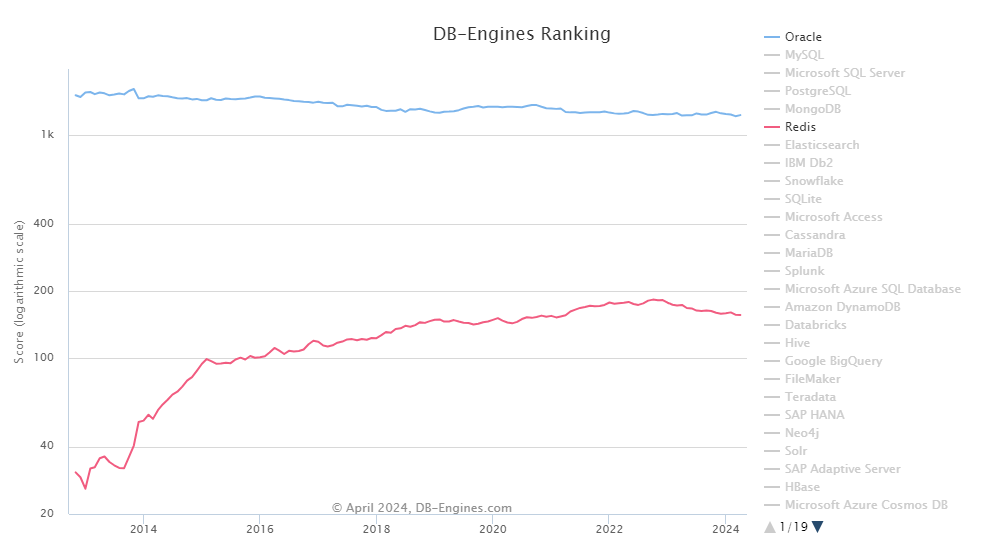
\includegraphics[scale=0.4]{Figures/db-engine-trend-dbs.PNG}
			\caption{Graf hodnot popularity RDBS Oracle a KDBS Redis~\cite{dbranking-trend-by-dbs}\label{graf-dbranking-trend-dbs}}
		\end{figure}
	\end{frame}
	
	\begin{frame}
		\frametitle{RDBS vs KDBS}
		\begin{figure}
			\centering
			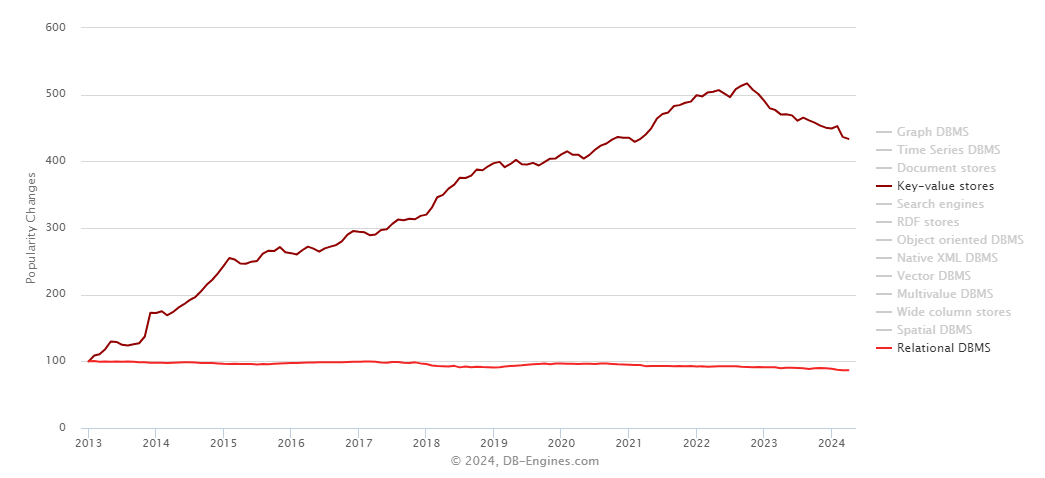
\includegraphics[scale=0.4]{Figures/db-engine-trend-model.PNG}
			\caption{Graf změn hodnot popularity RDBS a KDBS~\cite{dbranking-trend-by-model}}
		\end{figure}
	\end{frame}
	
	\begin{frame}
		\frametitle{KDBS}
		\begin{itemize}
			\item Databáze párů klíč-hodnota libovolného formátu
			\item Klíč je unikátní identifikátor umožňující rychlý přístup k hodnotám
			\item Základní operace (get(k), insert(k,h), delete(k), update(k,h))~\cite{vsb-nerelacni-db}
		\end{itemize}	
	\end{frame}
	
	\begin{frame}
		\frametitle{KDBS - hodnota}		
		\begin{figure}
			\centering
			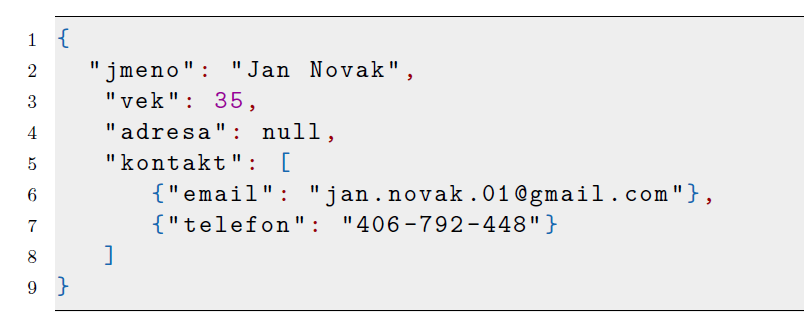
\includegraphics[scale=0.53]{Figures/hodnota_json.PNG}
			\caption{Hodnota (JSON dokument) uložená pro klíč "userid\_135"}
		\end{figure}
	\end{frame}
	
	\begin{frame}
		\frametitle{Testovací prostředí}
		\begin{itemize}
			\item Porovnání vlastností systémů (propustnost, bezpečnost, škálovatelnost)
			\item Nástroj pro nastavitelné a opakovatelné testy
			\item Řada nástrojů pro různorodé využití
			\item ApexSQL Diff, Apache JMeter, QuerySurge, Redgate SQL Test~\cite{dbs-testing-tools}
		\end{itemize}
	\end{frame}
	
	\begin{frame}
		\frametitle{TPC}
		\begin{itemize}
			\item Transaction Processing Performance Council (TPC)~\cite{tpc}
			\item Relační DBS
			\item Komplexní testování, náročné operace (agregace, seřazení, průměr, spojení) nad velkými daty
			\item Počet transakcí za minutu (tpm)
			\item TPC-C, TPC-H, TPCx-AI, TPCx-IoT, TPCx-BB
		\end{itemize}
	\end{frame}
	
	\begin{frame}
		\frametitle{TPC-H - SQL Test Q1}
		\begin{figure}
			\centering
			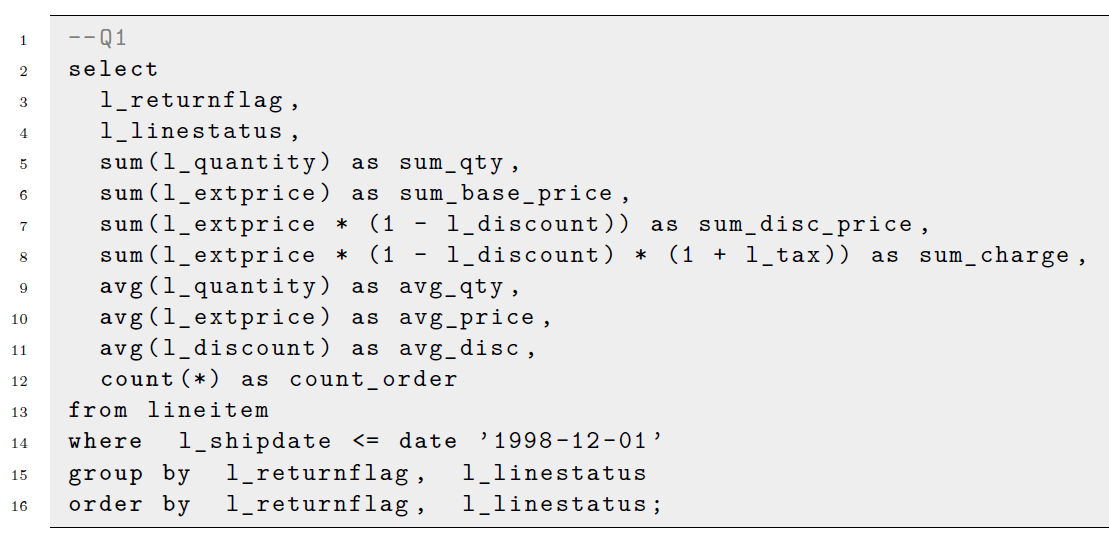
\includegraphics[scale=0.4]{Figures/tpc_test.PNG}
			\caption{TPC-H, SQL Test Q1~\cite{tpc-h-sql, tpc-h-index}}
		\end{figure}
	\end{frame}
	
	\begin{frame}
		\frametitle{YCSB}
		\begin{itemize}
			\item Yahoo! Cloud Serving Benchmark (YCSB)~\cite{ycsb}
			\item Porovnávání výkonu NoSQL DBS (KDBS)
			\item Scénáře využití (Workload A-F)
			\item Klíč - řetězec 'user\_id'
			\item Hodnota - JSON dokument s poli ('field0'-'fieldN')
		\end{itemize}
	\end{frame}
	
	\begin{frame}
		\frametitle{YCSB - operace vložení}
		\begin{figure}
			\centering
			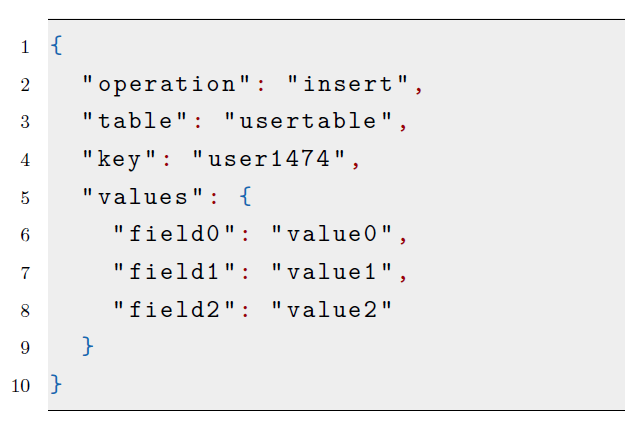
\includegraphics[scale=0.53]{Figures/ycsb_insert.PNG}
			\caption{YCSB - příklad definice operace vložení záznamu}
		\end{figure}
	\end{frame}
	
	\begin{frame}
		\frametitle{Zprovoznění testů}
		\begin{itemize}
			\item Java JDK 8 (1.8)~{\footnotesize\cite{java-jdk}}
			\item Nastavení \%JAVA\_HOME\% systémové proměnné~{\footnotesize\cite{win-env-var}} {\footnotesize(OS Windows)}
			\item Docker~{\footnotesize\cite{docker}}
			\item YCSB 0.17~{\footnotesize\cite{ycsb-download}}
			\item Apache Maven 3~{\footnotesize\cite{maven}}
			
		\end{itemize}
	\end{frame}

	\begin{frame}
		\frametitle{Zprovoznění testů - Docker}
		\begin{figure}
			\centering
			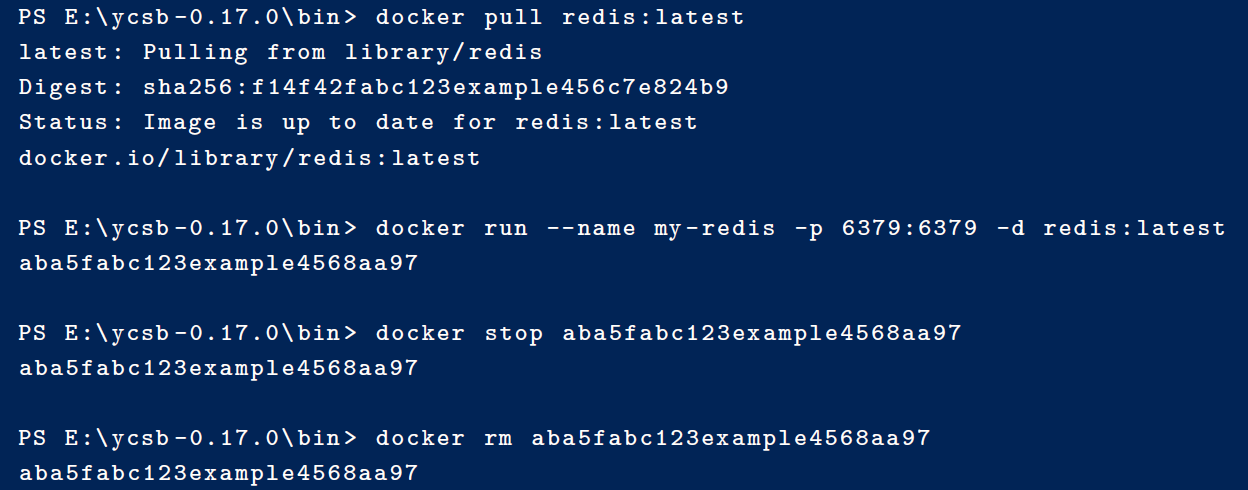
\includegraphics[scale=0.37]{Figures/docker_commands.PNG}
			\caption{Docker - příkazy pro stažení, spuštění, zastavení a odstranění DBS Redis}
		\end{figure}
	\end{frame}
	
	\begin{frame}
		\frametitle{Zprovoznění testů - YCSB Load}
		\begin{figure}
			\centering
			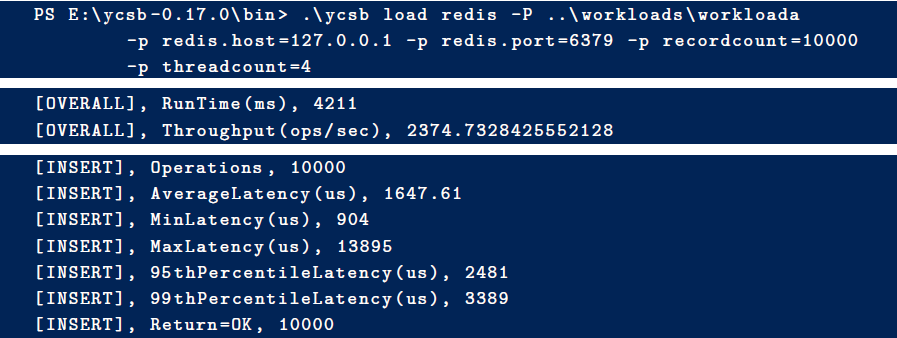
\includegraphics[scale=0.5]{Figures/ycsb_load_cut.PNG}
			\caption{YCSB Redis, příkaz pro vložení dat (load)}
		\end{figure}
	\end{frame}

	\begin{frame}
		\frametitle{Zprovoznění testů - YCSB Run}
		\begin{figure}
			\centering
			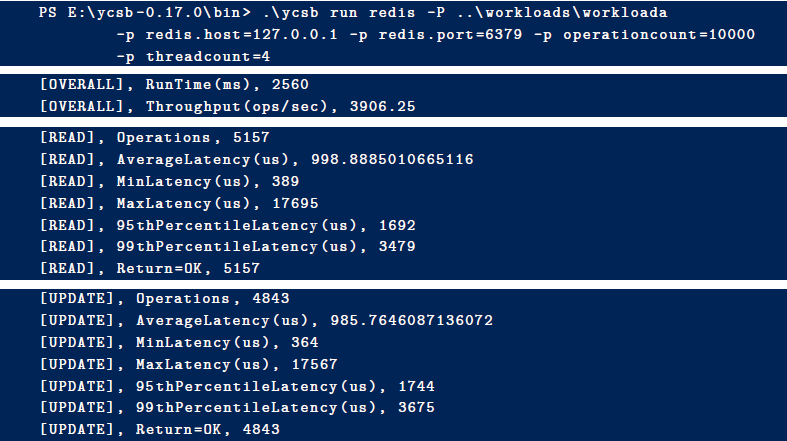
\includegraphics[scale=0.53]{Figures/ycsb_run_cut.PNG}
			\caption{YCSB Redis, příkaz pro spuštění testů (run)}
		\end{figure}
	\end{frame}
	
	\begin{frame}
		\frametitle{Parametry testů}
		\begin{itemize}
			\item Počet záznamů v databázi (recordcount)
			\item Počet testovaných operací (operationcount)
			\item Název DBS (Redis, Aerospike, Memcached, Riak KV)
			\item Workload A-C (readonly on/off)
			\item Případná konzistence (Riak KV měl chybně nastavenou silnou konzistenci)
		\end{itemize}
	\end{frame}
	
	\begin{frame}
		\frametitle{Spouštěcí skript}
		\begin{itemize}
			\item Windows PowerShell ISE (Integrované skriptovací prostředí)
			\item Automatizace, nahrazení ruční manipulace se skripty
			\item Docker, YCSB (specifikace cesty k bin adresáři)
			\item Výpis výsledků v příkazové řádce + textový soubor (složka Results)
		\end{itemize}
	\end{frame}
	
	\begin{frame}
		\frametitle{Spouštěcí skript - Ukázka}
		\begin{figure}
			\centering
			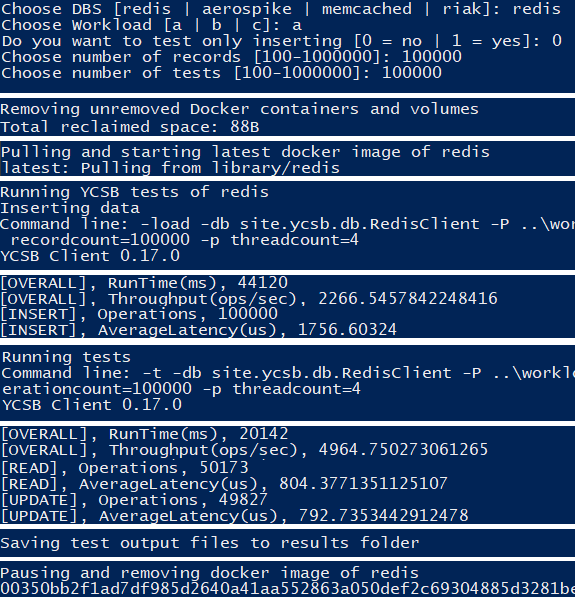
\includegraphics[scale=0.5]{Figures/tp_init.PNG}
		\end{figure}
	\end{frame}
	
	\begin{frame}
		\frametitle{Vyhodnocení testů - Workload A (50\% čtení, 50\% aktualizace)}
		\begin{figure}
			\begin{minipage}[b]{0.45\linewidth}
				\centering
				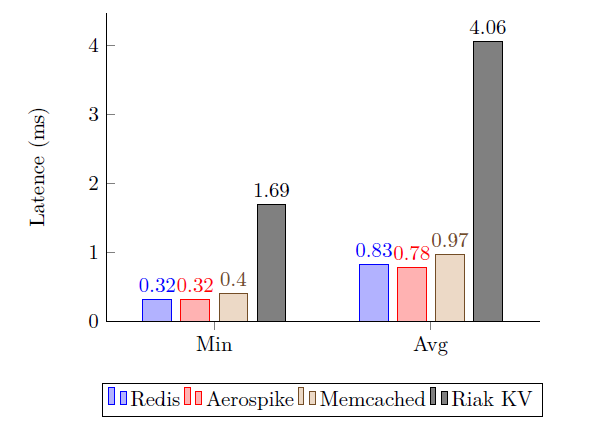
\includegraphics[width=\textwidth]{Figures/graf_wa_min_avg.PNG}
				\caption{Min a Avg latence (ms)}
			\end{minipage}
			\hspace{0.5cm}
			\begin{minipage}[b]{0.45\linewidth}
				\centering
				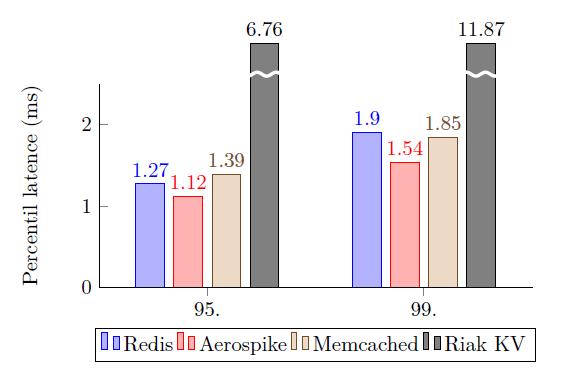
\includegraphics[width=\textwidth]{Figures/graf_perc.PNG}
				\caption{Percentil latence (ms)}
			\end{minipage}
		\end{figure}
	\end{frame}
	
	\begin{frame}
		\frametitle{Vyhodnocení testů - Propustnost (kops/sec)}
		\begin{figure}
			\centering
			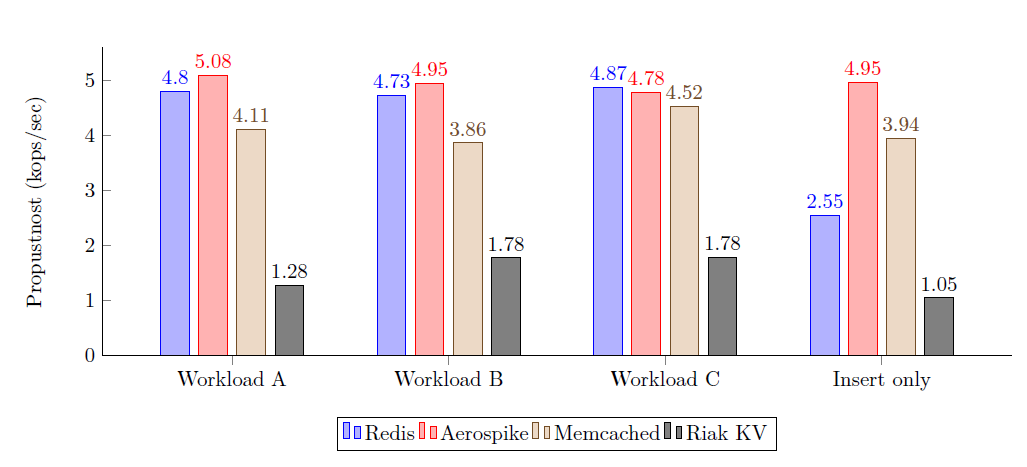
\includegraphics[scale=0.43]{Figures/graf_prop.PNG}
			\caption{Workload A, B, C + Insert only - Propustnost (kops/sec)}
		\end{figure}
	\end{frame}
	
	\begin{frame}
		\frametitle{Vyhodnocení testů - Souhrn}
		\begin{table}
			\centering
			\begin{tabular}{ l | c c c c }
				\hline
				Propustnost & 1. & 2. & 3. & 4. \\
				\hline
				Průměr všech & Aerospike & Redis & Memcached & Riak KV \\
				operací & 4,9 kops/s & 4,2 kops/s & 4,1 kops/s & 1,5 kops/s\\
				Vkládání & Aerospike & Memcached & Redis & Riak KV \\
				Aktualizace & Aerospike & Redis & Memcached & Riak KV \\
				Čtení & Redis & Aerospike & Memcached & Riak KV \\
				\hline
				\multicolumn{5}{c}{\tiny Na třetím řádku je uvedena průměrná propustnost všech testů (tisíce operací za sekundu) pro výše vypsaný KDBS} \\
			\end{tabular}
			\caption{Porovnání propustnosti výsledků testů}
		\end{table}
	\end{frame}
	
	\begin{frame}
		\frametitle{Riak KV, Silná konzistence (SC) vs Případná konzistence (EC)}
		\begin{figure}
			\centering
			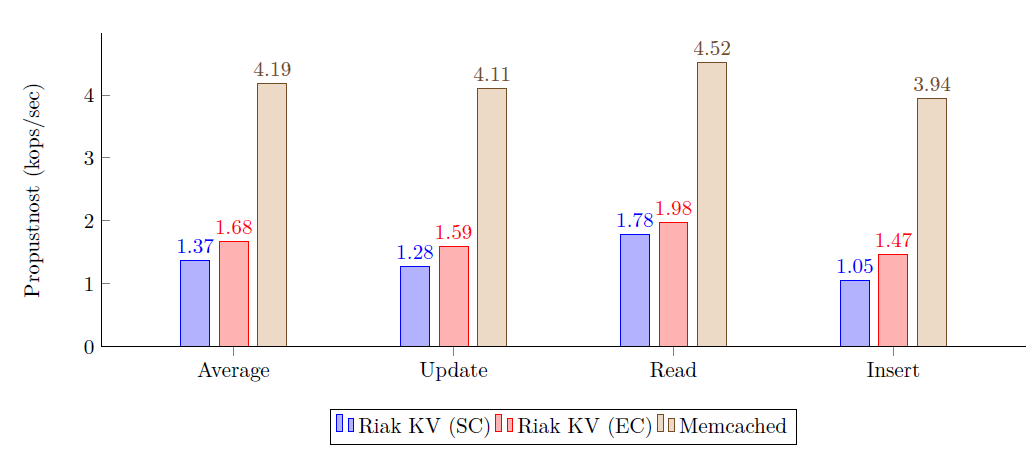
\includegraphics[scale=0.44]{Figures/riak_sc_ec.PNG}
			\caption{Riak KV SC vs EC - Propustnost (kops/sec), zlepšení o 22,6 \%}
		\end{figure}
	\end{frame}
	
	\begin{frame}
		\frametitle{Riak KV, Nízká propustnost}
		\begin{itemize}
			\item Přenastavení z SC na EC zvýšilo průměrnou propustnost o $\sim$310 operací za sekundu (22,6 \%), KDBS Memcached je stále rychlejší o 2,51 kops/sec (149,41 \%)
			\item Úplné vyřešení problému s chybou u operací aktualizace ($\sim$5 \%) přechodem na EC, nedochází ke konfliktům a operace nejsou zrušeny
			\item MapReduce je určen pro dávkové zpracování, nikoli pro dotazy v reálném čase
		\end{itemize}
	\end{frame}
	
	\begin{frame}[noframenumbering]
		\frametitle{Poděkování}
		\begin{center}
			\Huge
			Děkuji za pozornost
		\end{center}
	\end{frame}

	\begin{frame}[noframenumbering]
		\frametitle{Připomínky}
		\begin{itemize}
			\item Využití 4 vláken?
			\begin{itemize}
				\item Simulace paralelního provádění operací 4 klientů současně
				\item Více vláken nebylo použito skrz HW omezení stroje
			\end{itemize}
			\item Amazon DynamoDB úrovně izolace
			\begin{itemize}
				\item Podpora Read Uncommitted, Read Committed a Repeatable Reads
				\item Nepodporuje úroveň izolace Serializable
			\end{itemize}
			\item Redis datová struktura hash
			\begin{itemize}
				\item Redis hash - Hashovací tabulka
				\item Ideální pro objekty s řadou vlastností
			\end{itemize}
			\item Aerospike Hybrid-memory
			\begin{itemize}
				\item Index je v paměti, data na disku (nejedná se o In-memory)
				\item Při změně dat dojde k aktualizaci indexu v paměti a následně k zápisu změn na disk
				\item Index pro klíč uchovává metadata o lokaci záznamu na disku pro získání chybějících hodnot
			\end{itemize}
		\end{itemize}
	\end{frame}

	\begin{frame}[noframenumbering]
		\frametitle{Připomínky}
		\begin{itemize}
			\item Server-side clustering
			\begin{itemize}
				\item Dynamické nahrazení nedostupných serverů v rámci clusteru
				\item Horizontální škálovatelnost přidáním serverů do clusteru
			\end{itemize}
			\item Customer deployment
			\begin{itemize}
				\item Instalace, konfigurace a spuštění systému pro koncové uživatele
				\item Plánování, testování, implementace a podpora
			\end{itemize}
			\item Fail-over
			\begin{itemize}
				\item Dostupnost služeb při výpadku primárního serveru
				\item Přesun na záložní server či repliku při nedostupnosti primárního serveru
			\end{itemize}
			\item Hot-standby
			\begin{itemize}
				\item Poskytuje rychlý přechod a minimální dobu výpadku
				\item Hot-standby server je v reálném čase synchronizován s primárním serverem (okamžité replikování dat, dostupnost náhradní aktualizované kopie)
			\end{itemize}
		\end{itemize}
	\end{frame}

	\begin{frame}[noframenumbering,allowframebreaks]
		\frametitle{Citace}
		
		\printbibliography
		
	\end{frame}
	
\end{document}